\documentclass[12pt]{article}
\usepackage[utf8]{inputenc}
\usepackage{setspace}
\usepackage{graphicx}
\graphicspath{{images/}}
\usepackage{caption}
\doublespacing

\title {\textbf{Spectral Analysis In Linear Systems (SAILS)} \vspace{2 cm}}

\author{\huge \vspace{1.5 cm} Nazanin Rezajooei \\ \vspace{1 cm} Instructor: Dr. James Munroe \vspace{3 cm}\\  Department of chemistry \\ Memorial University \\ Newfoundland and Labrador}
\date{August 2020}


\begin{document}
\maketitle

\begin{abstract}
 The Fourier Transform can be defined as a tool that breaks a waveform (a function or signal) into an alternate representation, characterized by sine and cosines. In other words, The Fourier Transform is a mathematical technique that transforms a function of time, $X(t)$, to a function of frequency, $X(\omega)$. SAIL (Spectral Analysis In Linear Systems) is a package that transforms a function of time and signal into frequency. 
\end{abstract}

\section{Introduction}
\subsection{Autoregressive model}

The autoregressive model is defined as a model if it predicts future values based on past values.
As Eq.\ref{Eq:AR(1)} demonstrated,  the autoregressive model specifies that the output variable depends linearly on its previous values and stochastic terms. The order of an autoregression is the number of immediately preceding values in the series that are used to predict the value at present. So, the Eq. \ref{Eq:AR(1)} is a first-order autoregression model, written as AR(1). Eq.\ref{Eq:AR(2)} is a second-order autoregression model, written as AR(2), because the value at time $t$ is predicted from the values at times $t_1$ and $t_2$.

\begin{equation}
    y_t = \beta_0 + \beta_1 y_{t_1} + \epsilon_t
    \label{Eq:AR(1)}
\end{equation}

\begin{equation}
    y_t = \beta_0 + \beta_1 y_{t_1} + \beta_2 y_{t_2} + \epsilon_t
    \label{Eq:AR(2)}
\end{equation}

\subsection{Fourier transfer}

One of the essential things in this century is to discover the relation of data and analyze it in detail. Methods based on the Fourier transform have a vast application in all areas of science and engineering. Fourier transform is used in signal processing, for solving differential equations, or for analyzing the market dynamics. This method helps us understand information hidden in the time domain because it will appear in the frequency domain. For example, the MP3 and JPEG algorithms are based on transforming the time domain signal to the frequency domain signal. In this case, it is possible to make some process on the frequency domain signal, such as deleting the unimportant components and returning it to the time domain to reduce its size without affecting its quality \cite{F}.

\section{Methods}
\subsection{Data}

The Fourier transform allows you to transform a function of time and signal into frequency and power. This tells you what frequencies make up your signal and how strong they are. In our case, the signal is the number of phone calls, and we might be expecting some weekly or daily frequencies. Real data often contain noise, and the Fourier transform lets us see through the noise and see which frequencies matter. The data can be download from Kaggle, https://www.kaggle.com/mchirico/montcoalert .

After the data preparation, the first week and all-time data are plotted, and it can be seen in Fig. \ref{fig:data}. Some seasonality can be seen here, so it looks like our analysis will be promising. 

\begin{figure}[h]
    \centering
    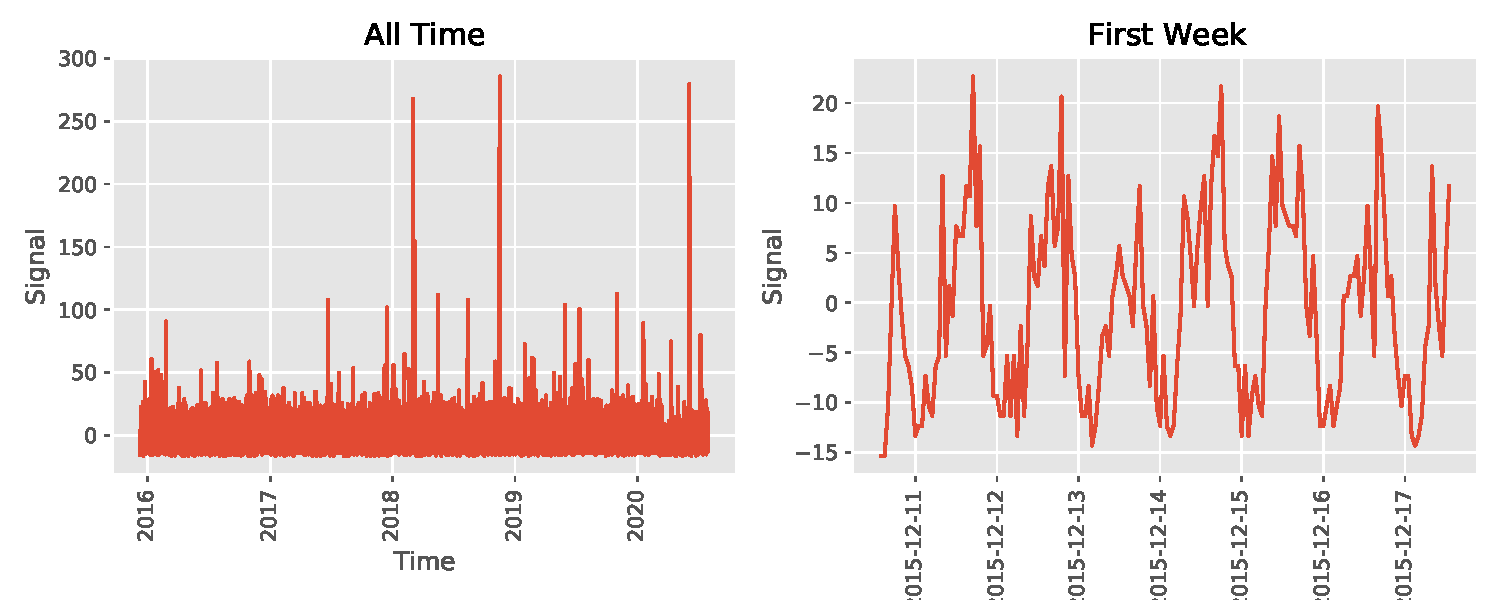
\includegraphics[scale = 0.55]{data.pdf}
    \caption{The all time and first week of signal}
    \label{fig:data}
\end{figure}

\subsection{Workflow}
Three steps implemented the project. First, the row data should be downloaded. The second step is data preparation, which pandas is used in this step. The third step is using the SAIL package to analyze the data and visualizing it.  

\subsection{Spectral Analysis In Linear Systems (SAILS)}

SAILS (Spectral Analysis in Linear Systems) is a python package that provides a basis for both the straightforward fitting of AR models as well as the exploration and development of newer methods, such as the decomposition of autoregressive parameters into eigenmodes.There are some packages, which implement multivariate regression fits including numpy.linalg and statsmodels.tsa. SAILS is extensible to work with model fits from other packages by creating a class inheriting from AbstractLinearModel and implementing the fit method to call the external package \cite{SAILS}.



\section{Results}

Just pass your input data into the function, and it’ll output the results of the transform. For the amplitude, take the absolute value of the results. As indicated in Fig.\ref{fig:fourier}, the frequencies with the highest amplitude are indicative of seasonal patterns. Frequencies with low amplitude are noise.

\begin{figure}[h]
    \centering
    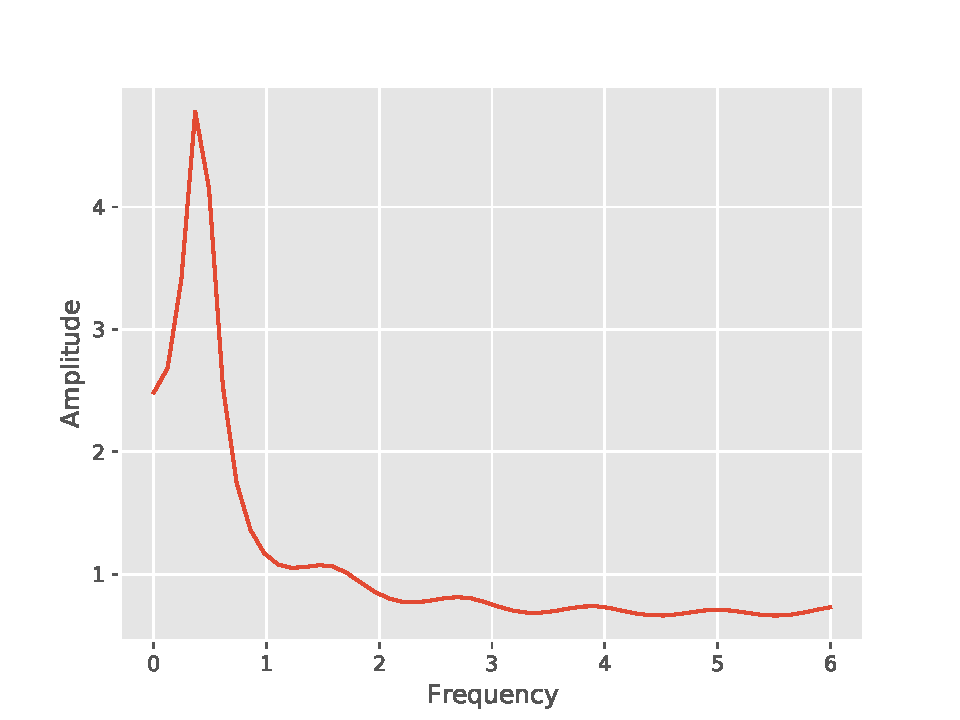
\includegraphics[scale = 0.6]{fourier.pdf}
    \caption{Showing the highest and lowest amplitude}
    \label{fig:fourier}
\end{figure}
\newpage
\bibliographystyle{unsrt}
\bibliography{ref.bib}

\end{document}
